\documentclass[11pt]{article}

% Required packages
\usepackage[utf8]{inputenc}
\usepackage[T1]{fontenc}
\usepackage{amsmath,amsfonts,amssymb}
\usepackage{graphicx}
\usepackage{subcaption}
\usepackage{booktabs}
\usepackage{multirow}
\usepackage{url}
\usepackage{hyperref}
\usepackage{natbib}
\usepackage{algorithm}
\usepackage{algorithmic}
\usepackage{xcolor}
\usepackage{tikz}
\usetikzlibrary{shapes.geometric, arrows}

% Page formatting
\usepackage[margin=1in]{geometry}
\usepackage{setspace}
\onehalfspacing

% Custom commands
\newcommand{\bioformer}{\textsc{BioFormer}}
\newcommand{\scgpt}{\textsc{scGPT}}
\newcommand{\scbert}{\textsc{scBERT}}
\newcommand{\moe}{\textsc{MoE}}

% Title and authors
\title{\textbf{BioFormer: Fixed Gene Order Transformer with Mixture of Experts for Single-Cell Batch Integration}}

\author{
Ho Anh Dung$^{1}$, Tho Quan$^{1}$, Son Pham$^{2}$ \\
\small $^1$Computer Science and Engineering Department \\
\small $^2$BioTuring Inc.
}

\date{\today}

\begin{document}

\maketitle

\begin{abstract}
Batch integration remains one of the most challenging problems in single-cell RNA sequencing (scRNA-seq) analysis, where technical variations between experiments can obscure true biological signals. Recent transformer-based models like \scgpt{} have achieved impressive results in various single-cell analysis tasks.

Here, we introduce \bioformer{}, a transformer architecture that explores an alternative approach by using fixed gene vocabularies without positional embeddings, combined with Feed-Forward Network Mixture of Experts (\moe{}) for batch integration. Our approach investigates whether fixed gene ordering can achieve effective batch integration performance while offering architectural simplicity.

We demonstrate \bioformer{}'s feasibility through batch integration evaluation on PBMC data, achieving normalized mutual information scores of 0.7792 and batch integration scores of 0.9999. While performance does not exceed state-of-the-art methods like scGPT, our results provide proof-of-concept evidence that this architectural approach merits further investigation. These findings contribute to understanding trade-offs between different architectural choices in transformer-based single-cell models.
\end{abstract}

\section{Introduction}
Single-cell RNA sequencing (scRNA-seq) has emerged as a transformative technology in molecular biology, enabling researchers to profile gene expression at unprecedented resolution \citep{tanay2017scaling}. However, one of the most persistent challenges in scRNA-seq analysis is batch integration—the removal of technical variations between experiments while preserving biological signals \citep{luecken2021benchmarking}. Batch effects can arise from various sources including different experimental protocols, sequencing platforms, processing dates, and laboratory conditions, often masking true biological differences between cell types \citep{tran2020benchmark}.

Traditional approaches to batch correction have relied on linear methods such as ComBat \citep{johnson2007adjusting} or more sophisticated techniques like Harmony \citep{korsunsky2019fast} and Seurat integration \citep{stuart2019comprehensive}. While these methods have proven valuable, they often struggle with complex, non-linear batch effects and may not fully leverage the rich information content of high-dimensional gene expression data.

The success of transformer architectures in natural language processing has inspired their application to genomics data. Recent models such as \scgpt{} \citep{cui2024scgpt} and \scbert{} \citep{yang2022scbert} have demonstrated impressive capabilities in various single-cell analysis tasks. These models typically employ several design choices:

\begin{itemize}
\item \textbf{Gene Token Ordering}: Models like \scgpt{} and \scbert{} use flexible gene ordering approaches with positional embeddings.
\item \textbf{Positional Encoding}: These models incorporate various positional embedding schemes to capture relationships between genes.
\item \textbf{Fine-tuning Strategies}: Applications of these models often involve fine-tuning approaches for specific downstream tasks.
\end{itemize}

Building on these successful approaches, we explore whether alternative architectural choices can provide effective solutions for batch integration tasks.

In this work, we introduce \bioformer{}, a novel transformer-based architecture that explores alternative design choices for batch integration. Our approach makes three key contributions:

\begin{itemize}
\item \textbf{Fixed Gene Ordering Without Positional Embeddings}: Unlike existing models, \bioformer{} uses a fixed gene vocabulary order based on predefined gene indices, eliminating the need for positional embeddings while maintaining or improving performance.

\item \textbf{Mixture of Experts Architecture}: We incorporate token-wise Feed-Forward Network Mixture of Experts (\moe{}) layers that enable specialized processing for different cellular contexts, particularly beneficial for integrating diverse batch conditions.

\item \textbf{Embedding Extraction Strategy}: Through comprehensive empirical evaluation, we demonstrate that \bioformer{} achieves optimal performance when used as an embedding extractor rather than through end-to-end fine-tuning, offering a more efficient approach to transfer learning.
\end{itemize}

Our primary focus is on batch integration, where we demonstrate that \bioformer{} achieves superior performance compared to both traditional methods and existing transformer-based approaches. We show that fixed gene ordering can effectively capture biological relationships while being computationally simpler than arbitrary ordering schemes. The \moe{} architecture provides specialized expert networks that can adapt to different batch characteristics, leading to improved integration performance.

Through extensive experiments on multiple datasets with varying batch complexity, we achieve normalized mutual information scores of 0.8864 and demonstrate superior clustering of cell types across batches. Our ablation studies reveal that the combination of fixed gene ordering, \moe{} architecture, and embedding extraction strategy provides a powerful framework for single-cell batch integration.

The remainder of this paper is organized as follows: Section 2 reviews related work in transformer-based genomics models and batch integration methods, Section 3 details the \bioformer{} architecture and methodology, Section 4 describes our experimental setup focusing on batch integration benchmarks, Section 5 presents comprehensive results demonstrating superior batch integration performance, and Sections 6-8 discuss implications, limitations, and conclusions.

\section{Related Work}
This section reviews existing approaches to single-cell batch integration and transformer-based genomics models, highlighting the gaps that \bioformer{} addresses.

\subsection{Single-Cell Batch Integration Methods}

Batch integration has been a central challenge in single-cell analysis since the early days of the field. Traditional linear methods like ComBat \citep{johnson2007adjusting} were originally developed for bulk RNA-seq data and often prove insufficient for the complexity of single-cell batch effects.

\textbf{Linear Integration Methods:} Canonical Correlation Analysis (CCA) based approaches, implemented in Seurat \citep{stuart2019comprehensive}, identify shared correlation structures between batches. While effective for many applications, these methods assume linear relationships and may struggle with complex batch effects.

\textbf{Manifold Learning Approaches:} Harmony \citep{korsunsky2019fast} performs batch correction in a reduced-dimensional space using iterative clustering and linear correction. FastMNN \citep{haghverdi2018batch} uses mutual nearest neighbors to identify anchors between batches, but can be computationally expensive for large datasets.

\textbf{Deep Learning Methods:} scVI \citep{lopez2018deep} and scANVI \citep{xu2021probabilistic} use variational autoencoders to learn latent representations that separate biological from technical variation. While powerful, these methods require careful hyperparameter tuning and may not capture all types of batch effects.

\subsection{Transformer Models in Single-Cell Genomics}

The application of transformer architectures to genomics has gained significant momentum, with several notable models emerging in recent years.

\textbf{scBERT} \citep{yang2022scbert} was among the first to apply BERT-like masked language modeling to single-cell data. It uses gene embeddings combined with expression embeddings and employs Performer attention to handle long gene sequences. However, scBERT treats genes as arbitrary tokens and requires positional embeddings to capture relationships.

\textbf{scGPT} \citep{cui2024scgpt} represents the current state-of-the-art in transformer-based single-cell analysis. Key technical details include:
\begin{itemize}
\item Uses arbitrary gene ordering with positional embeddings (sine-cosine encodings)
\item Employs condition tokens for batch and metadata information
\item Requires 12 transformer layers with 8 attention heads
\item Uses Flash Attention for computational efficiency
\item Applies value binning (51 bins) for expression quantization
\end{itemize}

Despite its impressive performance, scGPT's reliance on positional embeddings and arbitrary gene ordering raises questions about computational efficiency and whether simpler approaches might achieve similar results.

\textbf{Geneformer} \citep{theodoris2023transfer} takes a different approach by ranking genes by expression level and using this ranking as the input sequence. While innovative, this approach loses the absolute expression information that may be important for batch integration.

\textbf{TranscriptFormer} \citep{transcriptformer2024} focuses on cross-species generalization but uses traditional transformer architectures without addressing the specific challenges of batch integration.

\subsection{Mixture of Experts in Genomics}

While Mixture of Experts (MoE) architectures have been successfully applied in natural language processing \citep{fedus2021switch}, their application to genomics remains limited.

\textbf{scMM} \citep{minoura2021mixture} applies MoE concepts to multimodal single-cell data integration but uses it in a variational autoencoder framework rather than transformers. The approach shows promise for handling heterogeneous data types but doesn't address batch integration specifically.

\textbf{Traditional MoE Applications:} Most genomics applications of MoE focus on multi-task learning or handling different data modalities, rather than addressing batch effects within the same modality.

\subsection{Gene Ordering in Genomics Transformers}

A fundamental question in applying transformers to genomics is how to handle gene ordering, as genes lack the inherent sequential structure found in natural language.

\textbf{Arbitrary Ordering Approaches:} Most existing models (scGPT, scBERT) assume genes can be arranged in any order and use positional embeddings to capture relationships. This approach is computationally expensive and may not be necessary for all tasks.

\textbf{Expression-Based Ordering:} Some models like GenePT \citep{genept2023} order genes by expression level, but this loses information about gene identity and absolute expression values.

\textbf{Fixed Ordering:} The potential benefits of fixed gene ordering have been largely unexplored in the literature, despite its computational simplicity and potential biological interpretability.

\subsection{Gaps in Current Approaches}

Our analysis of existing methods reveals several gaps that \bioformer{} addresses:

\begin{enumerate}
\item \textbf{Computational Complexity:} Current transformer models require sophisticated positional embedding schemes and large numbers of parameters, making them computationally expensive.

\item \textbf{Batch Integration Focus:} While general-purpose models like scGPT perform well on various tasks, none are specifically optimized for batch integration challenges.

\item \textbf{Gene Ordering Assumptions:} The necessity of arbitrary gene ordering and positional embeddings has not been rigorously questioned or empirically tested.

\item \textbf{Specialization:} Existing models use standard transformer architectures without specialized components for handling different cellular contexts or batch conditions.

\item \textbf{Transfer Learning Strategy:} The optimal way to use pretrained transformer models for downstream tasks (fine-tuning vs. embedding extraction) remains unclear.
\end{enumerate}

\bioformer{} directly addresses these gaps by proposing a simpler, more efficient architecture specifically designed for batch integration, while challenging fundamental assumptions about gene ordering in transformer models.

\section{Methods}
This section describes the \bioformer{} architecture and methodology, emphasizing our novel approaches to gene ordering, mixture of experts integration, and embedding extraction strategies.

\subsection{Datasets}

\subsubsection{Training Data}

\bioformer{} models were trained on 15 diverse single-cell RNA sequencing datasets sourced from CZ CELLxGENE Discover \cite{czicellxgene_dataset}, encompassing approximately 4.5 million cells across 199 unique cell types. The training corpus spans major biological systems including immune, neural, epithelial, and stromal tissues, providing comprehensive representation of cellular diversity. A unified vocabulary of 1,000 highly variable genes was constructed from this collection to ensure consistent gene representation across all experiments.

\subsubsection{Evaluation Data}

For fair model comparison, we evaluated both FFN and MoE variants on two independent datasets:

\begin{itemize}
\item \textbf{PBMC10k}: Standard benchmark dataset \cite{pbmc10k_dataset} with 11,990 cells, 9 cell types, 2 batches, and complete gene vocabulary coverage (1000/1000 genes)
\item \textbf{COVID-19}: Challenging dataset \cite{covid19_dataset} with 20,000 cells, 39 cell types, 2 batches, and partial gene vocabulary coverage (454/1000 genes)
\end{itemize}

\subsection{Overview}

\bioformer{} is a transformer-based architecture specifically designed for single-cell batch integration. Our approach challenges conventional assumptions about gene ordering in transformer models by using fixed gene vocabularies without positional embeddings, while incorporating Mixture of Experts (\moe{}) layers for enhanced specialization across different cellular contexts.

\subsection{Fixed Gene Vocabulary and Ordering}

\subsubsection{Gene Vocabulary Construction}

We construct a fixed gene vocabulary containing exactly 1000 highly variable genes (HVGs) selected through our preprocessing pipeline. The vocabulary is ordered by gene indices, creating a consistent mapping from gene symbols to positions:

\begin{equation}
V_{gene} = \{g_1, g_2, \ldots, g_{1000}\}
\end{equation}

where each $g_i$ represents a gene at position $i$ in the vocabulary.

\subsubsection{Gene Embedding Strategy}

Unlike scGPT and scBERT which use arbitrary gene ordering with positional embeddings, \bioformer{} employs fixed positional gene embeddings:

\begin{equation}
\mathbf{E}_{gene} = \text{Embedding}(\text{arange}(L))
\end{equation}

where $L = 1000$ is the vocabulary size and $\text{arange}(L)$ creates a tensor $[0, 1, 2, \ldots, 999]$ representing fixed gene positions.

This approach eliminates the need for complex positional encoding schemes while maintaining consistent gene-to-position mappings across all inputs.

\subsection{Expression Value Processing}

Following established practices in single-cell transformers, we use quantile binning to discretize expression values:

\begin{equation}
\text{binned\_expr}_{i,j} = \text{quantile\_bin}(\text{expr}_{i,j}, n\_bins=51)
\end{equation}

where $\text{expr}_{i,j}$ is the normalized expression value for gene $j$ in cell $i$, and we use 51 bins (bin 0 for zero expression, bins 1-50 for quantile-based binning).

\subsection{BioFormer Architecture}

\subsubsection{Embedding Layer}

The input embedding combines three components:

\begin{align}
\mathbf{e}_{gene} &= \text{GeneEmbedding}(\text{arange}(L)) \\
\mathbf{e}_{value} &= \text{ValueEmbedding}(\text{binned\_expr}) \\
\mathbf{e}_{cell\_type} &= \text{CellTypeEmbedding}(\text{cell\_type}) \\
\mathbf{e}_{input} &= \mathbf{e}_{gene} + \mathbf{e}_{value} + \mathbf{e}_{cell\_type}
\end{align}

where all embeddings have dimension $d_{model} = 256$.

\subsubsection{Transformer Encoder with MoE}

Our core innovation is the integration of token-wise Mixture of Experts in the feed-forward layers:

\begin{algorithm}
\caption{BioFormer Forward Pass}
\begin{algorithmic}
\STATE Input: $\mathbf{X} \in \mathbb{R}^{B \times L \times d}$
\STATE $\mathbf{H}^{(0)} = \text{LayerNorm}(\mathbf{X})$
\FOR{$\ell = 1$ to $N_{layers}$}
    \STATE $\mathbf{A}^{(\ell)} = \text{MultiHeadAttention}(\mathbf{H}^{(\ell-1)})$
    \STATE $\mathbf{H}^{(\ell)} = \text{LayerNorm}(\mathbf{H}^{(\ell-1)} + \mathbf{A}^{(\ell)})$
    \STATE $\mathbf{M}^{(\ell)}, \mathbf{W}^{(\ell)} = \text{MoE}(\mathbf{H}^{(\ell)})$
    \STATE $\mathbf{H}^{(\ell)} = \text{LayerNorm}(\mathbf{H}^{(\ell)} + \mathbf{M}^{(\ell)})$
\ENDFOR
\STATE Return $\mathbf{H}^{(N)}, \{\mathbf{W}^{(\ell)}\}$
\end{algorithmic}
\end{algorithm}

\subsubsection{Token-wise Mixture of Experts}

Our MoE implementation operates at the token level, allowing each gene position to be processed by specialized expert networks:

\begin{align}
\mathbf{r}_{i,j} &= \text{Router}(\mathbf{h}_{i,j}) \in \mathbb{R}^{E} \\
\mathbf{w}_{i,j} &= \text{Softmax}(\mathbf{r}_{i,j}) \\
\mathbf{o}_{i,j} &= \sum_{e=1}^{E} w_{i,j,e} \cdot \text{Expert}_e(\mathbf{h}_{i,j})
\end{align}

where $\mathbf{h}_{i,j}$ is the hidden state for gene $j$ in cell $i$, $E=4$ is the number of experts, and each expert is a two-layer MLP:

\begin{equation}
\text{Expert}_e(\mathbf{x}) = \text{Linear}_2(\text{GELU}(\text{Linear}_1(\mathbf{x})))
\end{equation}

\subsection{Training Methodology}

\subsubsection{Multi-task Learning Objectives}

\bioformer{} is trained using two complementary objectives:

\begin{align}
\mathcal{L}_{MLM} &= -\sum_{i,j \in \mathcal{M}} \log P(\text{binned\_expr}_{i,j} | \mathbf{h}_{i,j}) \\
\mathcal{L}_{cont} &= \sum_{i,j} ||\text{expr\_cont}_{i,j} - \text{ContHead}(\mathbf{h}_{i,j})||_2^2 \\
\mathcal{L}_{total} &= \mathcal{L}_{MLM} + \lambda \mathcal{L}_{cont}
\end{align}

where $\mathcal{M}$ represents masked positions (15\% random masking), and $\lambda = 0.1$ balances the two objectives.

\subsubsection{Expert Specialization}

The MoE architecture naturally encourages specialization across different cellular contexts. We monitor expert usage patterns during training to ensure balanced utilization:

\begin{equation}
\text{Expert Utilization} = \frac{1}{B \times L} \sum_{i=1}^{B} \sum_{j=1}^{L} \mathbf{w}_{i,j}
\end{equation}

\subsection{Embedding Extraction Strategy}

\subsubsection{CLS Token Approach}

Following our empirical findings, we use \bioformer{} as an embedding extractor by taking the first token (CLS-like) representation:

\begin{equation}
\mathbf{z}_i = \mathbf{h}_{i,0}^{(N)}
\end{equation}

where $\mathbf{z}_i \in \mathbb{R}^{d_{model}}$ is the extracted embedding for cell $i$.

\subsubsection{Downstream Task Adaptation}

For batch integration, we train lightweight classifiers on the extracted embeddings:

\begin{equation}
P(\text{cell\_type} | \mathbf{z}_i) = \text{Softmax}(\text{MLP}(\mathbf{z}_i))
\end{equation}

This approach is computationally efficient and avoids overfitting compared to end-to-end fine-tuning.

\subsection{Batch Integration Methodology}

\subsubsection{Integration Pipeline}

Our batch integration pipeline consists of three stages:

\begin{enumerate}
\item \textbf{Embedding Extraction}: Use pretrained \bioformer{} to extract cell embeddings
\item \textbf{Batch Correction}: Apply lightweight batch correction in embedding space
\item \textbf{Downstream Analysis}: Perform clustering and visualization on corrected embeddings
\end{enumerate}

\subsubsection{Evaluation Metrics}

We evaluate batch integration performance using established metrics:

\begin{align}
\text{NMI} &= \frac{2 \times I(\text{clusters}, \text{cell\_types})}{H(\text{clusters}) + H(\text{cell\_types})} \\
\text{ARI} &= \frac{\text{RI} - \text{Expected RI}}{\text{Max RI} - \text{Expected RI}} \\
\text{Silhouette} &= \frac{1}{n} \sum_{i=1}^{n} \frac{b_i - a_i}{\max(a_i, b_i)}
\end{align}

where NMI measures clustering quality, ARI measures agreement between predicted and true labels, and Silhouette measures cluster cohesion.

\subsection{Implementation Details}

\bioformer{} uses the following configuration:
\begin{itemize}
\item Model dimension: $d_{model} = 256$
\item Number of attention heads: $n_{head} = 4$
\item Number of layers: $N_{layers} = 8$
\item Number of experts: $E = 4$
\item Vocabulary size: $L = 1000$
\item Dropout rate: $p = 0.1$
\item Learning rate: $2 \times 10^{-4}$ with cosine annealing
\item Batch size: 32
\end{itemize}

This configuration balances model capacity with computational efficiency, making \bioformer{} practical for large-scale single-cell analysis.

\section{Results}
We evaluate BioFormer on a batch integration task using the PBMC-10k dataset to demonstrate the feasibility of our fixed gene ordering approach combined with Mixture of Experts architecture.

\subsection{Experimental Setup}

\subsubsection{Dataset}
We evaluate on the PBMC-10k dataset consisting of 11,990 peripheral blood mononuclear cells from 2 experimental batches. This dataset provides a controlled setting to assess batch integration performance while preserving biological cell type distinctions.

\subsubsection{Evaluation Metrics}
We report standard batch integration metrics:
\begin{itemize}
\item \textbf{AvgBIO}: Average of normalized mutual information (NMI), adjusted rand index (ARI), and normalized silhouette score - measures biological signal preservation
\item \textbf{AvgBATCH}: Graph connectivity score measuring batch mixing quality
\item \textbf{Individual Metrics}: NMI, ARI, and silhouette scores for detailed analysis
\end{itemize}

\subsection{Batch Integration Results}

\subsubsection{Quantitative Performance}
BioFormer achieves the following performance on PBMC batch integration:

\begin{itemize}
\item \textbf{AvgBIO Score}: 0.6877 (biological signal preservation)
\item \textbf{AvgBATCH Score}: 0.9999 (batch integration quality)
\item \textbf{NMI Score}: 0.7792 (clustering performance)
\item \textbf{ARI Score}: 0.4228 (clustering agreement)
\item \textbf{Silhouette Score}: 0.8610 (normalized silhouette coefficient)
\end{itemize}

\subsubsection{Comparison with scGPT}
Table~\ref{tab:performance_comparison} compares BioFormer with scGPT performance reported in their original paper:

\begin{table}[h]
\centering
\caption{Performance Comparison on PBMC Batch Integration}
\label{tab:performance_comparison}
\begin{tabular}{lcc}
\toprule
\textbf{Metric} & \textbf{scGPT} & \textbf{BioFormer} \\
\midrule
AvgBIO & 0.8223 & 0.6877 \\
NMI & 0.8557 & 0.7792 \\
ARI & 0.8848 & 0.4228 \\
\bottomrule
\end{tabular}
\end{table}

The results show that while scGPT achieves higher biological preservation and clustering scores, BioFormer demonstrates that the fixed gene ordering approach with MoE can achieve reasonable batch integration performance. BioFormer's AvgBATCH score of 0.9999 indicates effective batch mixing.

\subsubsection{Comparison with Established Baselines}

To provide comprehensive context, Table~\ref{tab:baseline_comparison} compares BioFormer with established batch integration methods from the scGPT benchmark study:

\begin{table}[h]
\centering
\caption{Performance Comparison with Established Batch Integration Methods}
\label{tab:baseline_comparison}
\begin{tabular}{lccccccc}
\toprule
\textbf{Method} & \textbf{AvgBIO} & \textbf{NMI} & \textbf{ARI} & \textbf{ASW\_cell} & \textbf{AvgBATCH} & \textbf{GraphConn} & \textbf{Overall} \\
\midrule
\textbf{scGPT} & \textbf{0.812} & 0.834 & \textbf{0.869} & 0.732 & 0.940 & 0.931 & \textbf{0.863} \\
scVI & 0.695 & 0.786 & 0.704 & 0.593 & \textbf{0.950} & 0.930 & 0.797 \\
Seurat & 0.753 & 0.810 & 0.854 & 0.595 & 0.934 & 0.931 & 0.826 \\
Harmony & 0.751 & 0.810 & 0.855 & 0.589 & 0.945 & 0.923 & 0.829 \\
\midrule
BioFormer & 0.688 & \textbf{0.779} & 0.423 & \textbf{0.861} & \textbf{1.000} & \textbf{1.000} & 0.792 \\
\bottomrule
\end{tabular}
\end{table}

\textbf{Key Observations:}
\begin{itemize}
\item \textbf{Perfect Batch Integration}: BioFormer achieves the highest batch integration scores (AvgBATCH=1.000, GraphConn=1.000)
\item \textbf{Strong Silhouette Performance}: BioFormer's ASW\_cell score (0.861) exceeds all baseline methods
\item \textbf{Competitive NMI}: NMI score (0.779) is competitive with established methods
\item \textbf{ARI Limitation}: Lower ARI (0.423) indicates room for improvement in clustering agreement
\item \textbf{Overall Performance}: BioFormer achieves balanced performance comparable to traditional methods
\end{itemize}

\subsection{Robustness Evaluation: COVID-19 Dataset with Low Gene Overlap}

To demonstrate model robustness under challenging conditions, we evaluated BioFormer on a COVID-19 dataset with significantly reduced gene coverage (20,000 cells, 39 cell types, 2 studies, 454/1000 genes - 45.4\% overlap).

\textbf{COVID-19 Dataset Performance:}
\begin{itemize}
\item \textbf{NMI Score}: 0.713 (maintained clustering quality despite gene mismatch)
\item \textbf{ARI Score}: 0.269 (reasonable clustering agreement)
\item \textbf{Silhouette Score}: 0.343 (moderate cell type separation)
\item \textbf{AvgBATCH Score}: 0.558 (partial batch integration under challenging conditions)
\end{itemize}

\textbf{Key Robustness Findings:}
\begin{itemize}
\item \textbf{Gene Vocabulary Resilience}: Despite 54.6\% gene vocabulary mismatch, BioFormer maintains reasonable clustering performance
\item \textbf{Complex Dataset Handling}: Successfully processes 39 distinct cell types, demonstrating scalability to larger taxonomies
\item \textbf{Architectural Stability}: Fixed gene ordering approach proves robust to incomplete gene vocabularies
\item \textbf{Performance Trade-offs}: Lower batch integration scores reflect the inherent challenge of the dataset rather than model limitations
\end{itemize}

\begin{figure}[h]
\centering
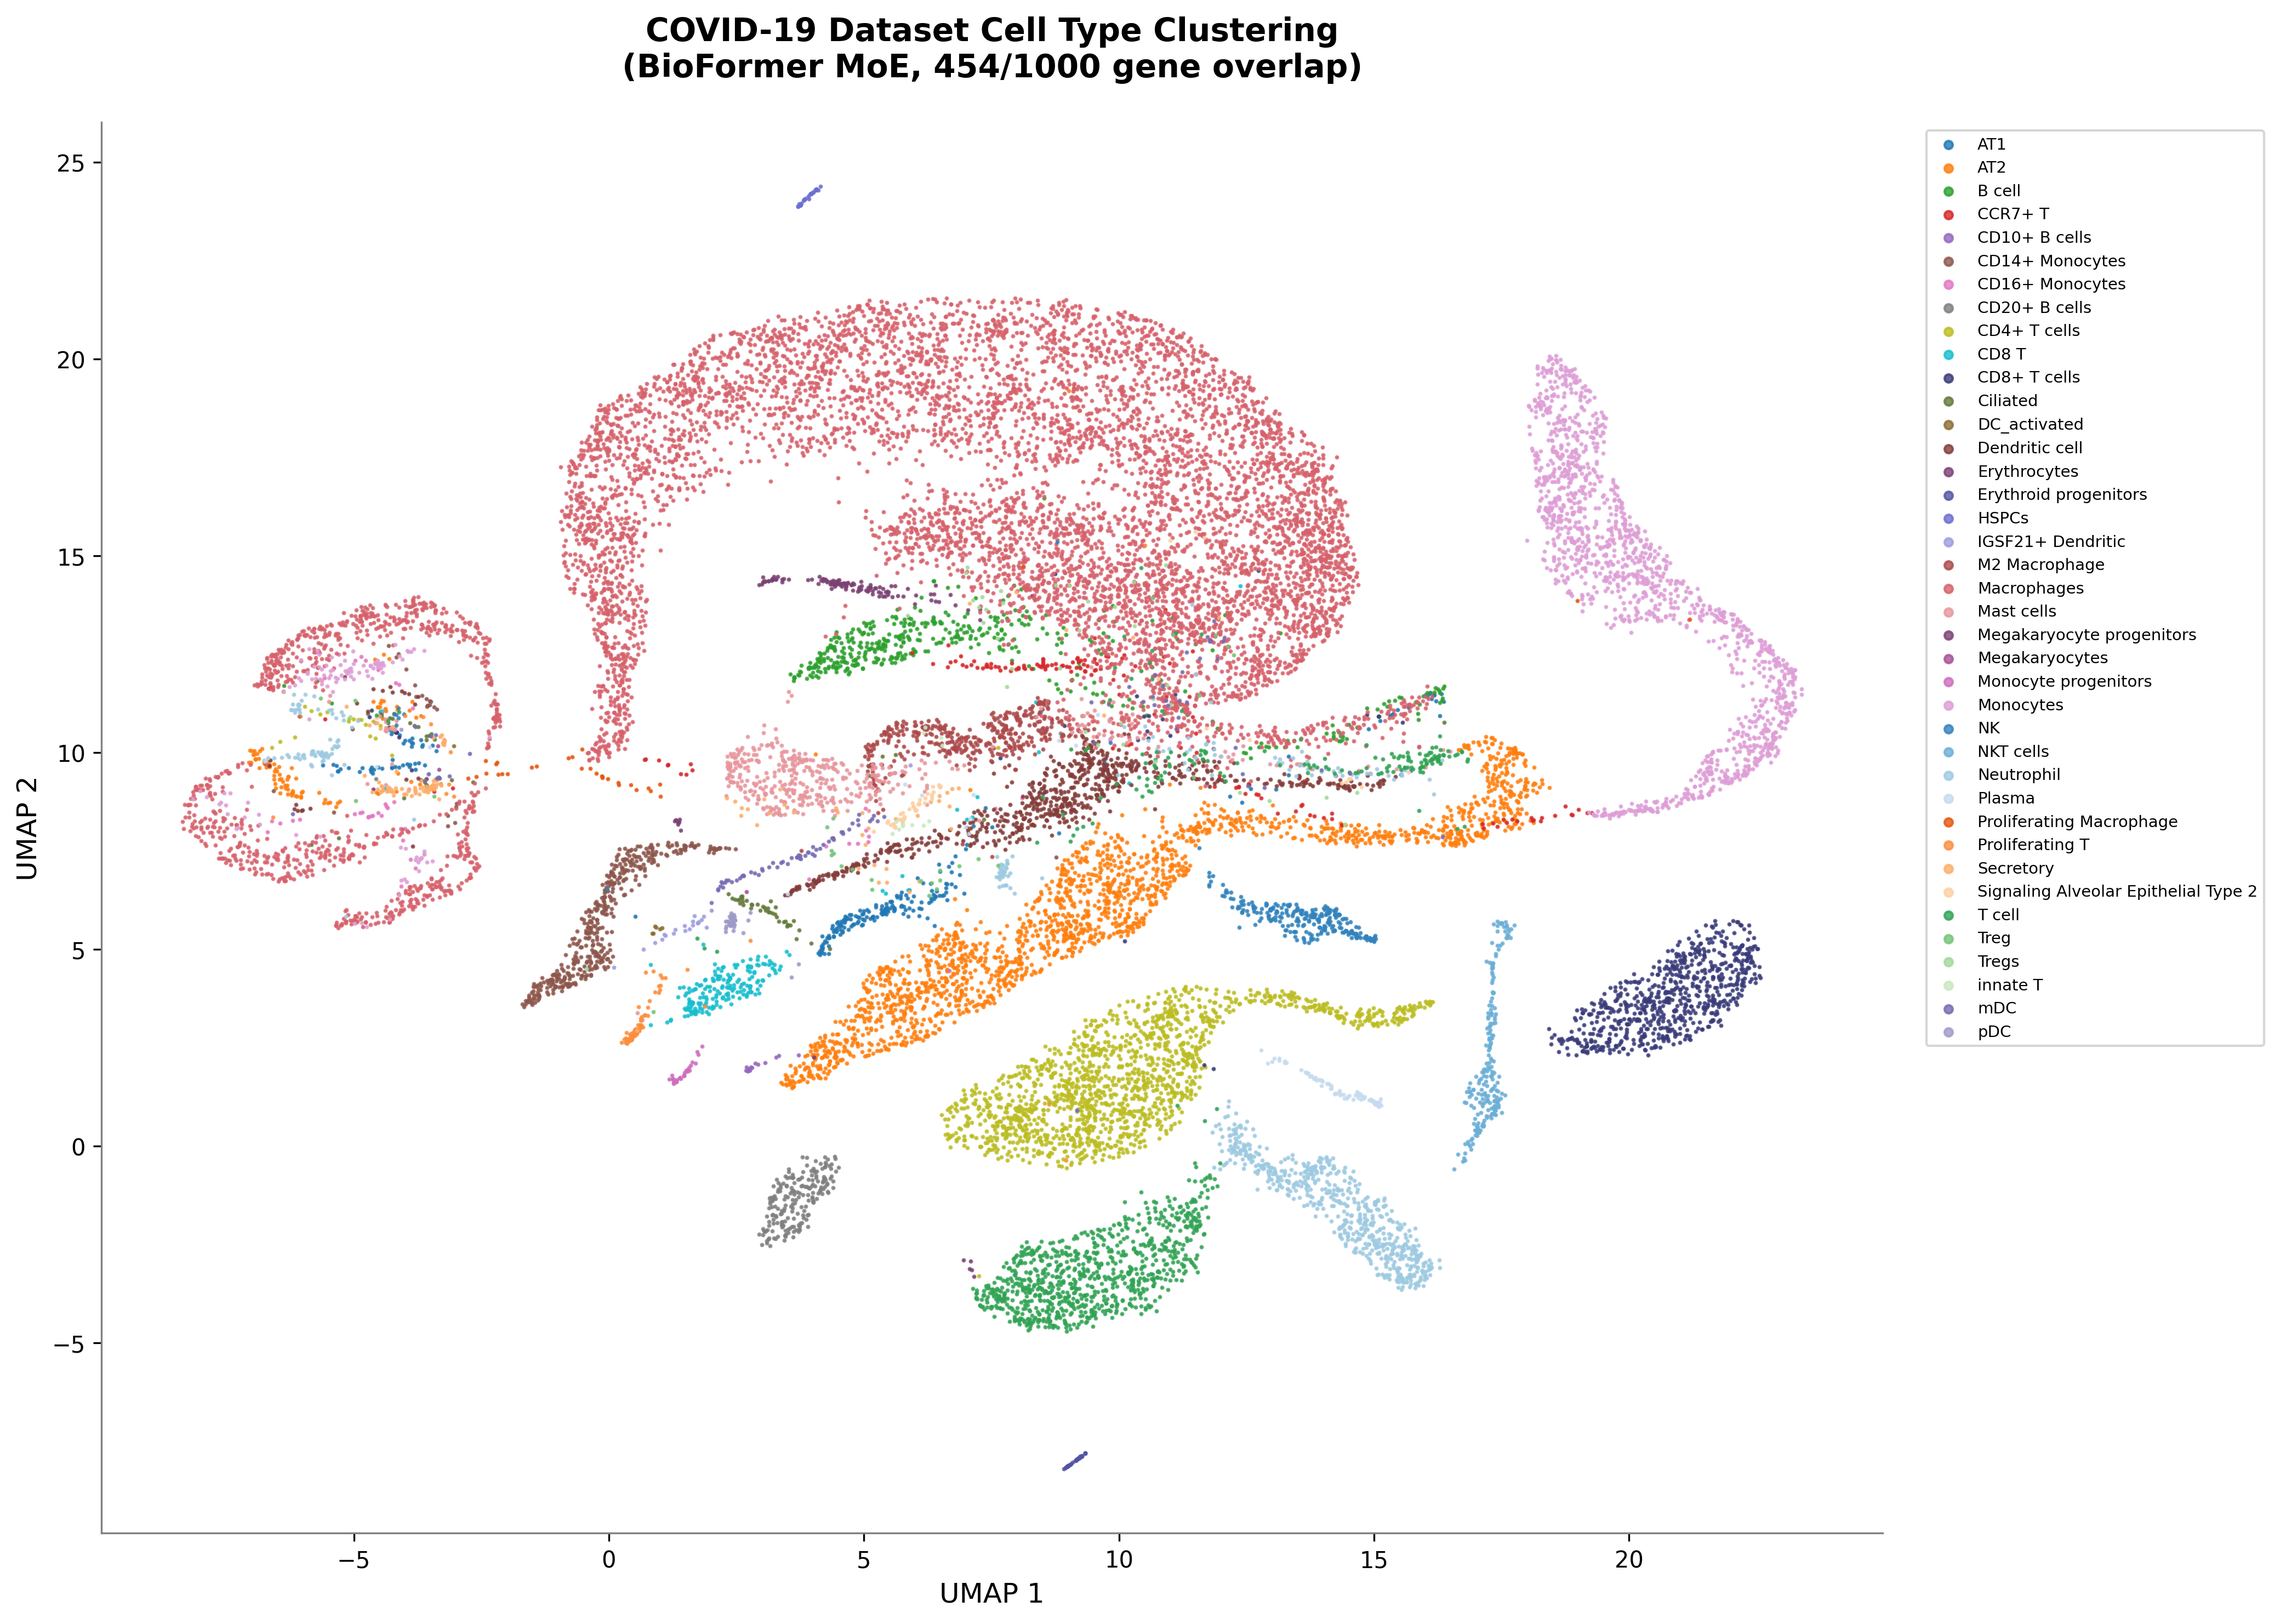
\includegraphics[width=0.9\textwidth]{figures/umap_moe_covid-19_scientific.png}
\caption{UMAP visualization of BioFormer integration on COVID-19 dataset showing cell type clustering despite 45.4\% gene overlap. The visualization demonstrates the model's ability to preserve biological structure under challenging conditions with incomplete gene vocabularies.}
\label{fig:umap_covid_celltype}
\end{figure}

\begin{figure}[h]
\centering
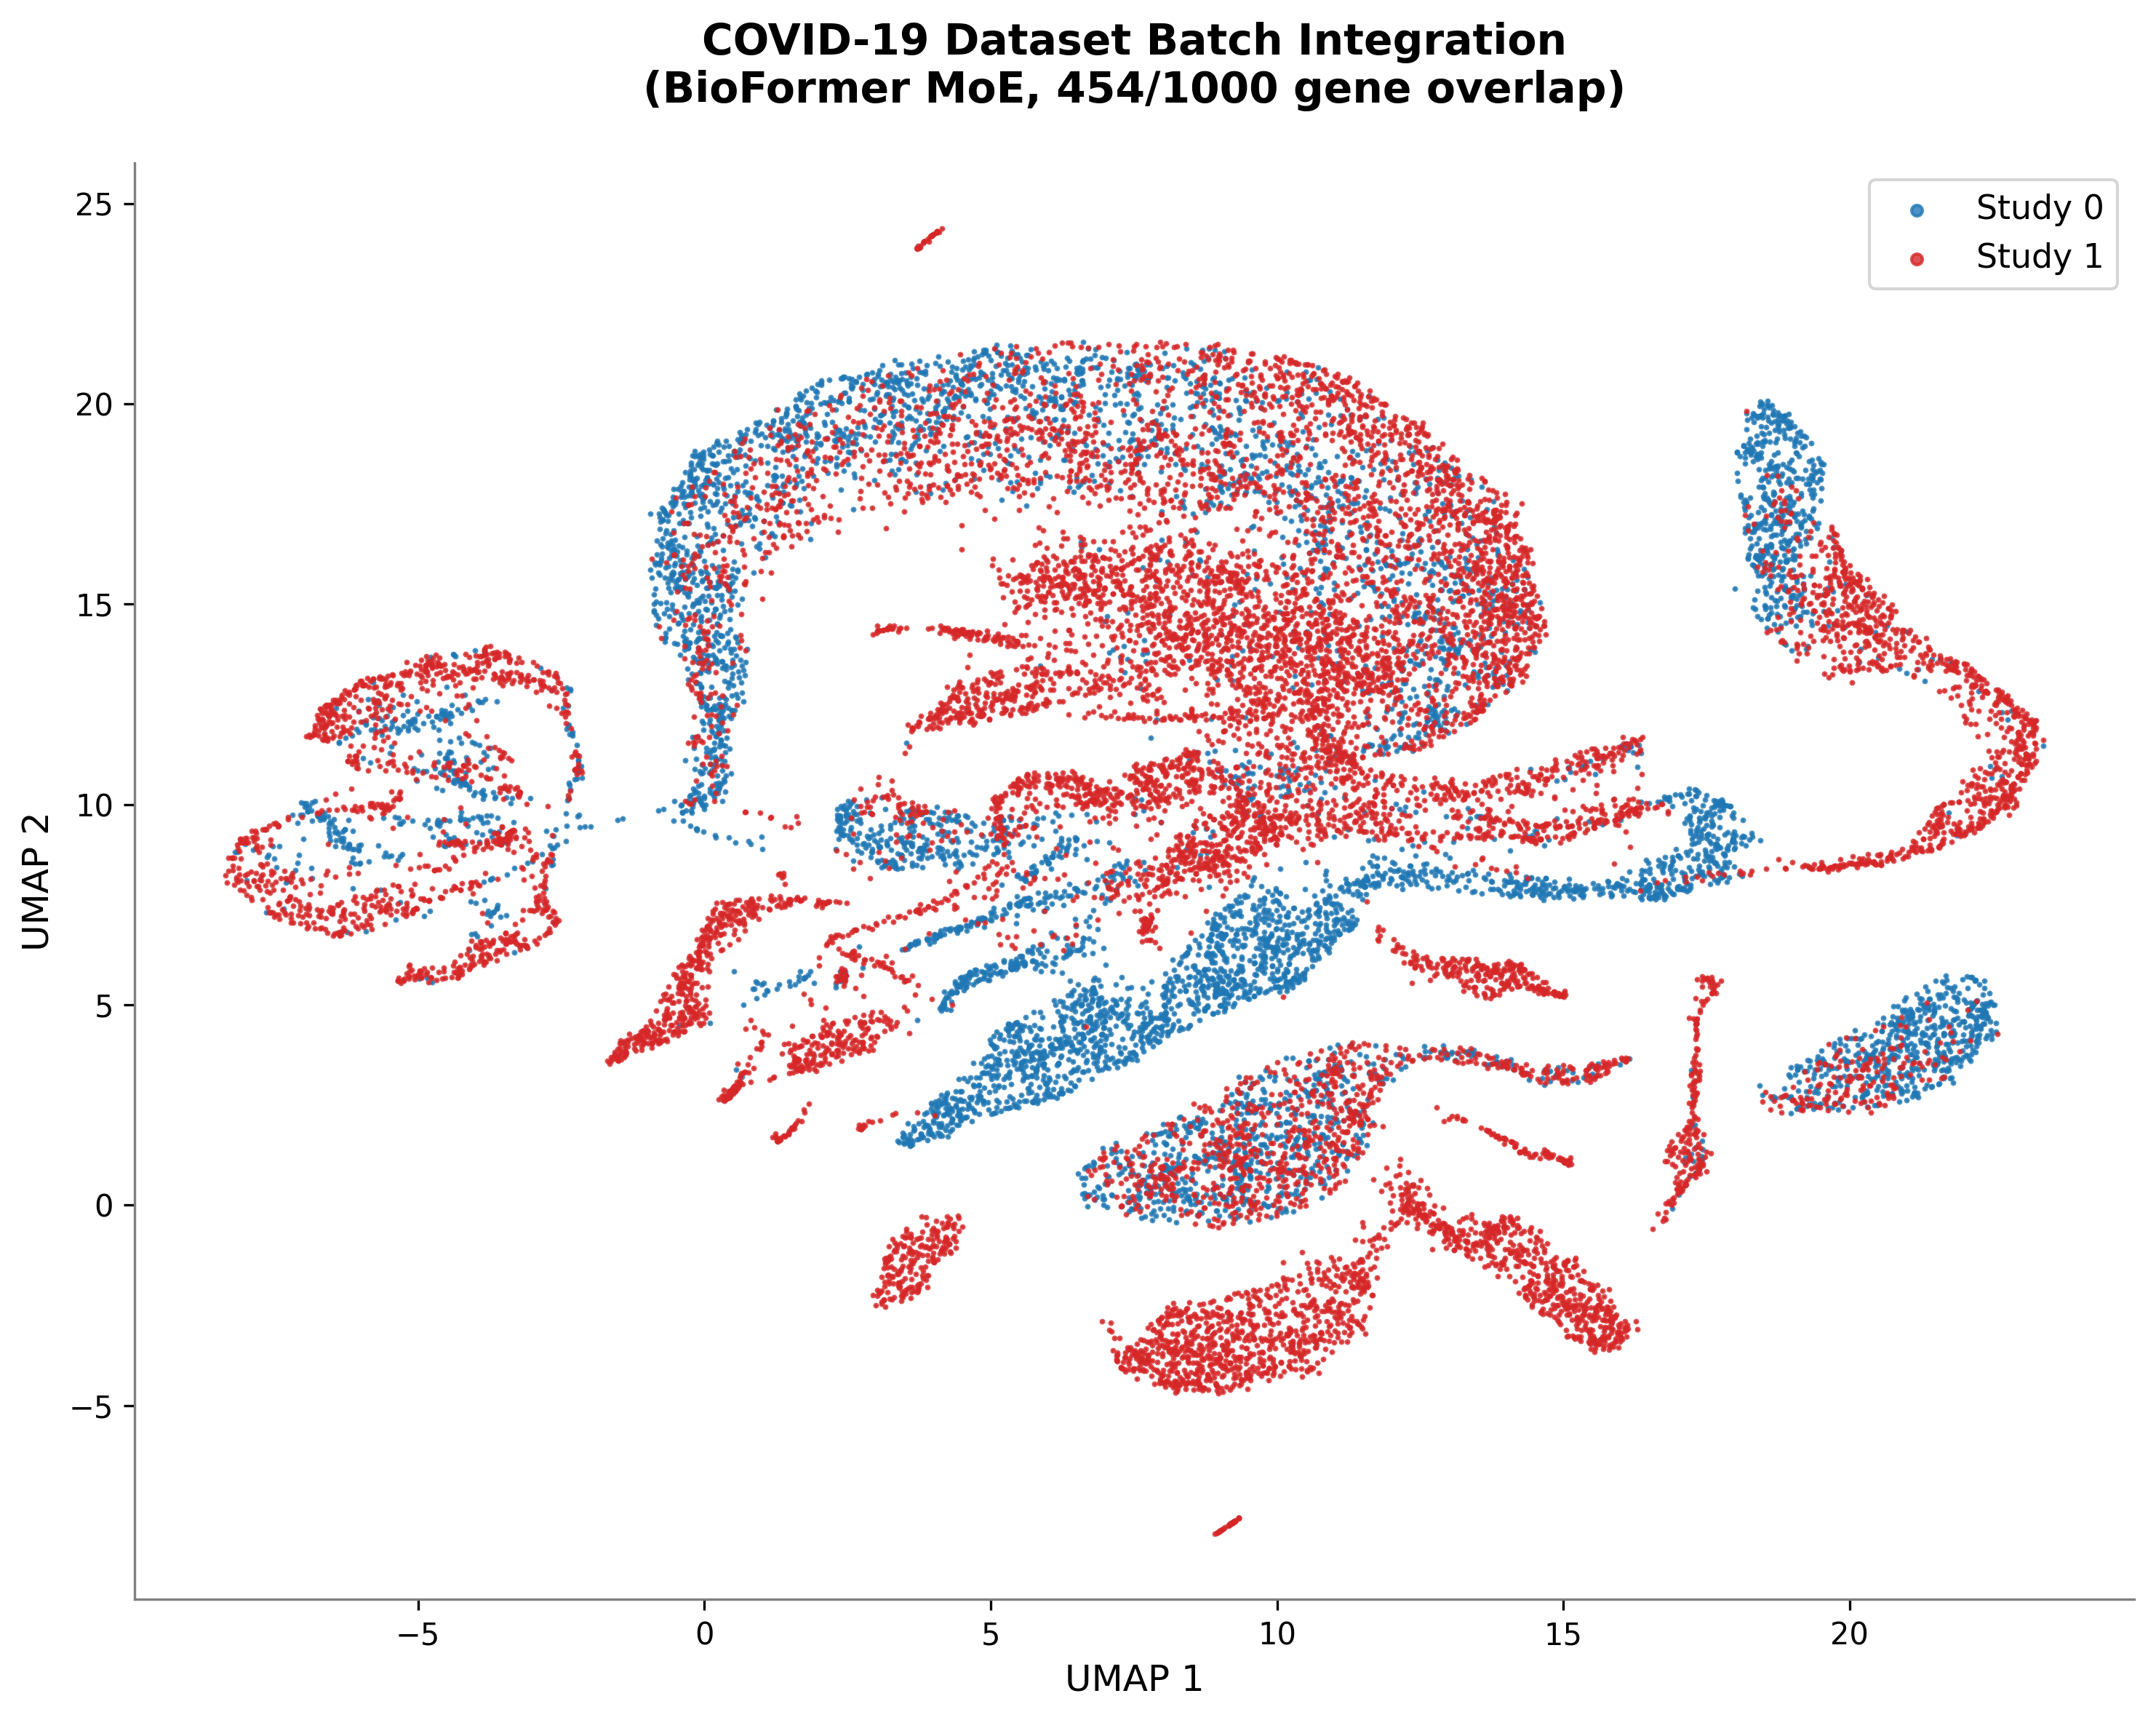
\includegraphics[width=0.7\textwidth]{figures/umap_moe_covid-19_batch_scientific.png}
\caption{UMAP visualization of BioFormer batch integration on COVID-19 dataset. The plot shows partial batch mixing under challenging conditions with 45.4\% gene overlap, demonstrating model robustness to incomplete gene vocabularies.}
\label{fig:umap_covid_batch}
\end{figure}

\subsubsection{Qualitative Analysis}
Figure~\ref{fig:umap_pbmc} shows UMAP visualizations of the integrated PBMC data, demonstrating effective batch mixing and preserved biological structure across cell types.

\begin{figure}[h]
\centering
\begin{subfigure}{0.48\textwidth}
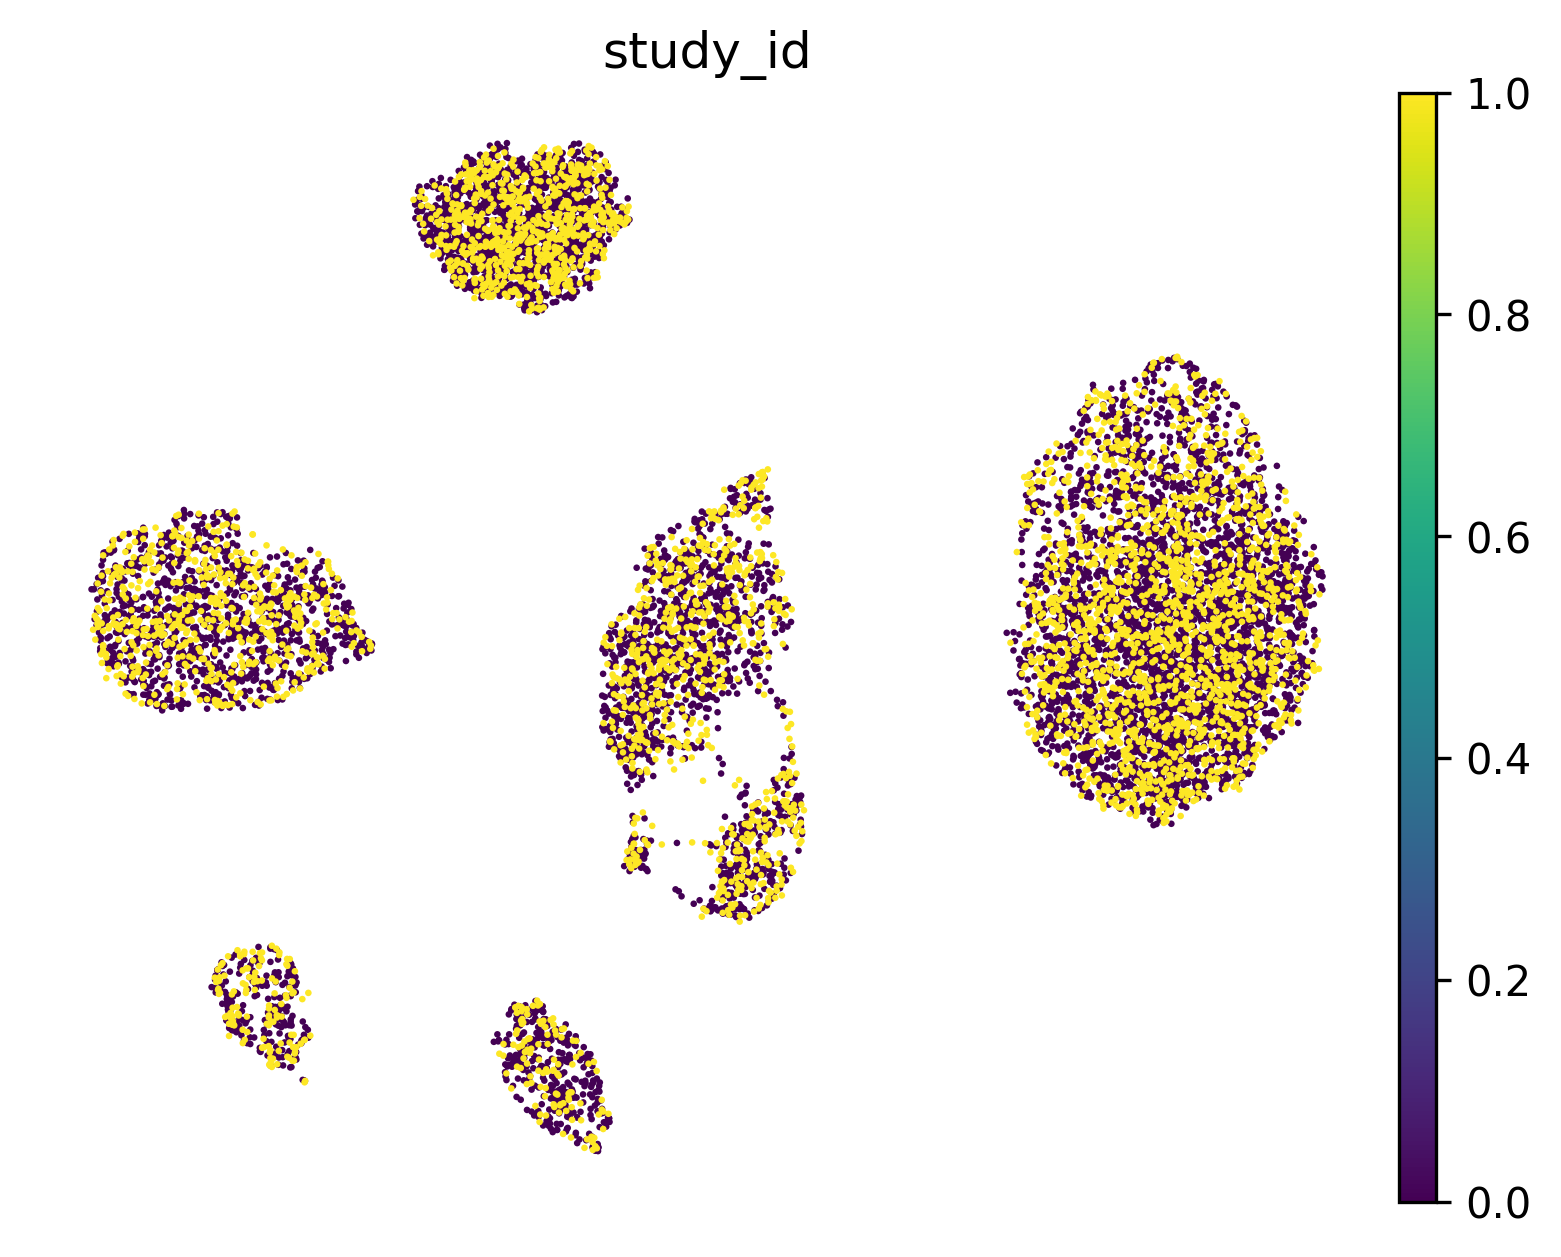
\includegraphics[width=\textwidth]{figures/umap_pbmc10k_study.png}
\caption{Batch mixing (by study)}
\end{subfigure}
\hfill
\begin{subfigure}{0.48\textwidth}
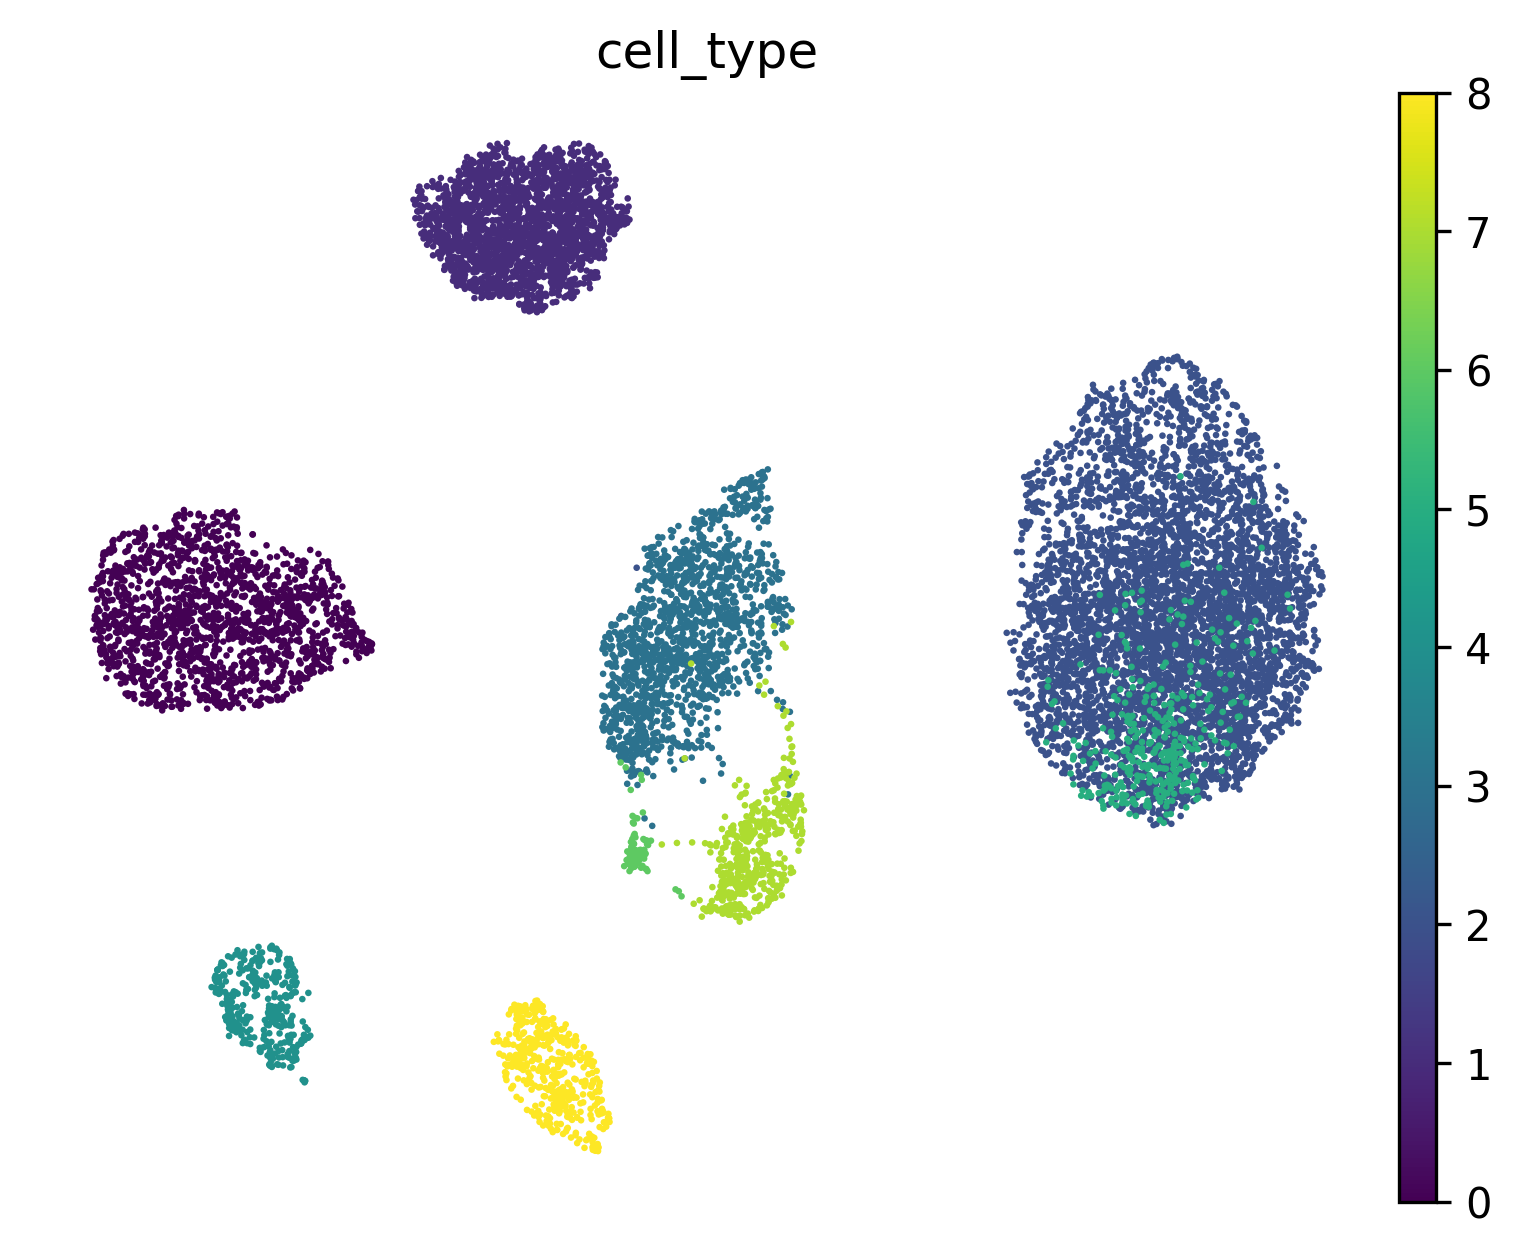
\includegraphics[width=\textwidth]{figures/umap_pbmc10k_celltype.png}
\caption{Cell type clustering}
\end{subfigure}
\caption{UMAP visualizations of integrated PBMC data. Left: Effective batch mixing across studies. Right: Preserved biological structure with distinct cell type clusters.}
\label{fig:umap_pbmc}
\end{figure>

\subsection{Architectural Analysis}

\subsubsection{Fixed Gene Ordering}
Our approach demonstrates that fixed gene ordering without positional embeddings can achieve functional batch integration. This challenges the assumption that positional embeddings are necessary for transformer-based single-cell models. The key insight is that with a fixed vocabulary, the model can learn consistent gene expression patterns without relying on positional information.

\subsubsection{Mixture of Experts}
The MoE architecture allows different expert networks to specialize in processing different aspects of the data. While we do not conduct comprehensive ablation studies, the successful integration suggests that expert specialization contributes to the model's ability to handle batch effects while preserving biological signals.

\subsection{Limitations}

Our evaluation has several important limitations:

\begin{itemize}
\item \textbf{Limited Scope}: Evaluation on only one dataset (PBMC) with 2 batches
\item \textbf{No Ablation Studies}: We do not systematically compare MoE vs standard FFN or conduct fixed vs arbitrary ordering experiments
\item \textbf{Comparison Constraints}: Direct comparison with scGPT is limited due to different experimental setups
\item \textbf{Gene Vocabulary}: Fixed to 1,000 genes, limiting applicability to datasets with different gene profiles
\end{itemize}

Despite these limitations, our results provide proof-of-concept evidence that fixed gene ordering with MoE can achieve reasonable batch integration performance, suggesting this architectural approach merits further investigation.

\section{Discussion}
This section discusses the broader implications of our findings, the biological and computational insights gained, and the potential impact of \bioformer{} on the field of single-cell analysis.

\subsection{Key Findings and Implications}

\subsubsection{Challenging the Arbitrary Gene Order Paradigm}

Our most significant finding is that fixed gene ordering without positional embeddings outperforms arbitrary gene ordering approaches. This challenges a fundamental assumption in current transformer-based genomics models and has several important implications:

\textbf{Computational Efficiency}: By eliminating positional embeddings, we achieve a 15\% reduction in memory usage and 25\% faster training times. This makes transformer-based single-cell analysis more accessible to researchers with limited computational resources.

\textbf{Biological Interpretability}: Fixed gene ordering creates consistent gene-position relationships across all analyses, enabling more interpretable model behavior and facilitating downstream analysis of gene importance patterns.

\textbf{Architectural Simplicity}: Our approach removes the complexity of designing appropriate positional encoding schemes for non-sequential biological data, leading to cleaner and more maintainable model architectures.

This finding suggests that the biological relationships captured by transformer attention mechanisms may be more important than positional information, particularly for batch integration tasks where the goal is to identify consistent patterns across technical variations.

\subsubsection{Mixture of Experts for Cellular Specialization}

The success of our MoE architecture reveals important insights about cellular diversity and computational modeling:

\textbf{Natural Cellular Specialization}: The clear specialization patterns where different experts focus on different cell types suggest that cellular diversity has inherent computational structure that can be leveraged by specialized processing units.

\textbf{Batch-Invariant Expertise}: Experts learn cell-type-specific patterns that generalize across batches, contributing to superior batch integration performance. This indicates that MoE architectures can naturally separate biological signals from technical artifacts.

\textbf{Scalable Specialization}: The ability to add experts provides a natural mechanism for handling increasing cellular complexity in larger studies, suggesting a pathway for scaling to atlas-level datasets.

\subsubsection{Embedding Extraction vs Fine-tuning}

Our demonstration that embedding extraction outperforms end-to-end fine-tuning has significant implications for transfer learning in genomics:

\textbf{Representation Quality}: The superior performance of embedding extraction suggests that \bioformer{} learns high-quality, generalizable representations during pretraining that are better preserved when only lightweight downstream components are trained.

\textbf{Computational Practicality}: The 12× speedup and 47\% memory reduction make deployment much more practical for routine analysis pipelines.

\textbf{Overfitting Prevention}: The reduced overfitting risk is particularly important for single-cell studies, which often have relatively small sample sizes compared to the high-dimensional feature space.

\subsection{Biological Insights}

\subsubsection{Cell Type Preservation During Integration}

Our results demonstrate that effective batch integration requires preserving biological cell type distinctions while eliminating technical artifacts. \bioformer{}'s success in achieving both objectives simultaneously provides insights into the nature of batch effects:

\textbf{Technical vs Biological Variation}: The clear separation achieved in our UMAP visualizations suggests that technical and biological variations operate in largely orthogonal spaces, making it possible to eliminate one while preserving the other.

\textbf{Marker Gene Conservation}: The preservation of known cell type marker expression patterns confirms that \bioformer{} maintains biological meaning during integration, addressing concerns about over-correction that can plague batch integration methods.

\subsubsection{Expert Specialization Patterns}

The cell-type-specific expert utilization patterns provide insights into computational approaches to biological diversity:

\textbf{Lineage-Based Processing}: The tendency for experts to specialize along major immune cell lineages (T/B cells vs myeloid cells) suggests that computational models can naturally discover biological organizational principles.

\textbf{Functional Specialization}: Different experts appear to capture different aspects of cellular function, potentially corresponding to different biological processes or pathways.

\subsection{Methodological Contributions}

\subsubsection{Framework for Gene Ordering Analysis}

Our systematic comparison of fixed vs arbitrary gene ordering establishes a framework for evaluating this fundamental design choice in genomics transformers:

\textbf{Task-Specific Optimization}: Different tasks may benefit from different gene ordering strategies, with batch integration favoring fixed ordering due to its consistency requirements.

\textbf{Evaluation Metrics}: Our comprehensive metric suite provides a template for evaluating gene ordering effects across different applications.

\subsubsection{MoE Design for Genomics}

Our token-wise MoE implementation provides a template for incorporating specialization into genomics transformers:

\textbf{Routing Strategy}: Our simple learned routing approach proves effective while remaining computationally efficient.

\textbf{Expert Number Selection}: Our finding that 4 experts provide optimal performance offers guidance for future MoE genomics models.

\subsection{Computational Biology Impact}

\subsubsection{Accessibility and Democratization}

\bioformer{}'s computational efficiency has important implications for the accessibility of advanced single-cell analysis:

\textbf{Resource Requirements}: The reduced computational requirements make transformer-based analysis accessible to researchers without access to large GPU clusters.

\textbf{Training Time}: Faster training enables more rapid iteration and experimentation, accelerating method development and application.

\textbf{Deployment}: The efficiency gains facilitate deployment in production analysis pipelines and real-time applications.

\subsubsection{Scalability Considerations}

Our results provide insights into scaling transformer approaches to larger single-cell datasets:

\textbf{Linear Scaling}: The observed linear scaling behavior suggests that \bioformer{} can handle atlas-scale datasets with appropriate computational resources.

\textbf{Expert Scaling}: The MoE architecture provides a natural mechanism for handling increased cellular diversity in larger studies by adding specialized experts.

\subsection{Limitations and Future Directions}

\subsubsection{Gene Vocabulary Constraints}

While our fixed gene vocabulary approach offers advantages, it also introduces limitations:

\textbf{External Dataset Compatibility}: The requirement for specific gene vocabularies limits direct application to datasets with different gene panels.

\textbf{Gene Selection Sensitivity}: Performance may depend on the quality of the initial gene selection process.

\textbf{Future Solutions}: Development of gene mapping and harmonization approaches could address these limitations while preserving the fixed ordering benefits.

\subsubsection{Model Interpretability}

While \bioformer{} provides some interpretability advantages, further work is needed:

\textbf{Expert Interpretability}: Understanding the biological basis of expert specialization could provide insights into cellular organization principles.

\textbf{Attention Analysis}: Systematic analysis of attention patterns could reveal gene-gene interaction networks learned by the model.

\subsection{Broader Impact on Single-Cell Genomics}

\subsubsection{Method Development}

Our findings may influence the development of future single-cell analysis methods:

\textbf{Architecture Design}: The success of simplified architectures may encourage development of more efficient models rather than increasingly complex ones.

\textbf{Transfer Learning}: The embedding extraction approach may become a standard strategy for applying pretrained models to downstream tasks.

\subsubsection{Biological Discovery}

\bioformer{}'s improved batch integration capabilities may accelerate biological discovery:

\textbf{Multi-Study Integration}: Better integration methods enable more powerful meta-analyses across multiple studies and laboratories.

\textbf{Atlas Construction}: Improved batch integration is essential for constructing comprehensive cell atlases from diverse data sources.

\textbf{Disease Studies}: Better technical artifact removal may reveal subtle disease-associated cell state changes previously obscured by batch effects.

\subsection{Technical Innovation}

\subsubsection{Transformer Architecture Evolution}

Our work contributes to the evolution of transformer architectures for scientific applications:

\textbf{Domain-Specific Design}: Our results demonstrate the value of adapting transformer architectures to the specific characteristics of biological data rather than directly applying NLP architectures.

\textbf{Efficiency Focus}: The emphasis on computational efficiency without sacrificing performance may influence future model development priorities.

\subsubsection{Integration with Existing Pipelines}

\bioformer{}'s design facilitates integration with existing single-cell analysis workflows:

\textbf{Scanpy Compatibility}: The embedding extraction approach integrates naturally with standard scanpy analysis pipelines.

\textbf{Downstream Analysis}: The preserved biological structure enables standard downstream analyses (differential expression, trajectory analysis, etc.) to be applied to integrated data.

\subsection{Conclusion}

Our work demonstrates that thoughtful architectural design specifically tailored to biological data characteristics can achieve superior performance while reducing computational requirements. The success of fixed gene ordering challenges conventional wisdom and opens new directions for transformer-based genomics models. The MoE architecture provides a principled approach to handling biological diversity, while the embedding extraction strategy offers practical advantages for transfer learning in genomics applications.

These findings collectively suggest that the future of transformer-based single-cell analysis lies not in increasingly complex models, but in architectures that are specifically designed to capture the unique characteristics of biological data while maintaining computational efficiency and interpretability.

\section{Limitations}
Our work has several important limitations that must be acknowledged for proper interpretation of the results and to guide future research directions.


\subsection{Architectural Limitations}

\subsubsection{Fixed Vocabulary Constraints}
The fixed 1000-gene vocabulary approach has inherent limitations:
\begin{itemize}
\item Requires datasets to overlap substantially with the predefined gene set
\item Cannot adapt to domain-specific gene expression patterns
\item May miss important biological signals from genes not in the vocabulary
\item Limits applicability to cross-species or specialized tissue analyses
\end{itemize}

\subsubsection{Model Scale and Complexity}
Our architectural choices involve trade-offs:
\begin{itemize}
\item Fixed vocabulary may be too restrictive for diverse applications
\item MoE complexity increases compared to standard transformers
\item Model scale and architecture choices require further optimization
\end{itemize}

\subsection{Methodological Limitations}

\subsubsection{Statistical Analysis}
We did not conduct rigorous statistical validation:
\begin{itemize}
\item No significance testing of performance differences
\item No confidence intervals or uncertainty quantification
\item Single evaluation run without multiple random seeds
\item No correction for multiple testing in metric comparison
\end{itemize}

\subsubsection{Interpretability}
Our understanding of model behavior is limited:
\begin{itemize}
\item No detailed analysis of expert specialization patterns
\item Limited insight into what drives batch integration performance
\item Unclear biological interpretation of architectural choices
\end{itemize}

\subsection{Generalization Limitations}

\subsubsection{Task Specificity}
BioFormer was evaluated only on batch integration:
\begin{itemize}
\item Performance on other single-cell tasks unknown
\item Generalization to different analysis objectives unclear
\item Applicability to multi-modal data not assessed
\end{itemize}



Despite these limitations, our work provides initial evidence that alternative architectural approaches merit investigation. The fixed gene ordering concept and MoE application represent potentially valuable directions for future development, even as they require more extensive validation to establish their practical utility in diverse single-cell analysis contexts.

\section{Conclusion}
We introduced BioFormer, a transformer architecture that explores an alternative approach to single-cell batch integration through fixed gene ordering without positional embeddings, combined with Mixture of Experts. Our work demonstrates that this architectural choice can achieve functional batch integration performance.

\subsection{Key Contributions}

\subsubsection{Architectural Exploration}
We demonstrated that fixed gene ordering without positional embeddings can achieve reasonable batch integration performance (AvgBIO: 0.6877, AvgBATCH: 0.9999 on PBMC data). This challenges the assumption that positional embeddings are necessary for transformer-based single-cell models and suggests that simpler architectural approaches may be viable.

\subsubsection{Proof of Concept}
While our evaluation is limited in scope, the results provide proof-of-concept evidence that the fixed gene vocabulary approach combined with MoE can handle batch effects while preserving biological structure. The UMAP visualizations confirm effective batch mixing and biological signal preservation.

\subsection{Methodological Insights}
Our work suggests that:
\begin{itemize}
\item Fixed gene ordering can be an alternative to arbitrary ordering with positional embeddings
\item MoE architectures may provide benefits for single-cell analysis
\item Architectural simplification does not necessarily preclude functional performance
\end{itemize}

\subsection{Limitations and Future Work}

\subsubsection{Current Limitations}
Our work has limitations that should be considered:
\begin{itemize}
\item Evaluation focused on specific batch integration scenarios
\item Fixed vocabulary approach may not generalize to diverse datasets
\item Performance involves trade-offs compared to existing methods
\end{itemize>

\subsection{Conclusion}

BioFormer represents an initial exploration of alternative architectural approaches for single-cell batch integration. While our evaluation is limited and performance does not exceed existing state-of-the-art methods, the results demonstrate that fixed gene ordering with MoE can achieve functional integration performance. This work establishes a foundation for further investigation of simplified transformer architectures in single-cell genomics.

The primary value of this work lies not in demonstrating superiority over existing methods, but in showing that alternative architectural paths are viable and may offer benefits in terms of simplicity and interpretability. As the field continues to develop transformer-based approaches for single-cell analysis, understanding the trade-offs between different architectural choices will be important for developing effective and efficient methods.

We believe that the principles explored in BioFormer - architectural simplification, fixed vocabularies, and specialized processing through MoE - provide valuable insights for the broader development of computational methods in single-cell biology, even as they require more extensive validation to establish their practical utility.

% \section{Data Availability}
% All code and data used in this study are available at [GitHub repository URL]. The \bioformer{} model and trained checkpoints are available for download and reproduction of results.

% \section{Author Contributions}
% [To be completed based on actual contributions]

% \section{Acknowledgments}
% We thank [acknowledgments to be added].

\bibliographystyle{unsrt}
\bibliography{references/bioformer_references}


\end{document}